\documentclass[../main.tex]{subfiles}

\makeatletter
\@ifundefined{fromRoot}{%
  \newcommand{\fromRoot}[1]{../#1}
  
  \usepackage{xr}
  \externaldocument{../main}
}{}

\def\input@path{{\subfix{../}}}
%or: \def\input@path{{/path/to/folder/}{/path/to/other/folder/}}
\makeatother

\graphicspath{
  {\subfix{../}}
  {\subfix{./figures}}
  {\subfix{../figures}}
  {\subfix{./figures/logos-thesis/}}
  {\subfix{../figures/logos-thesis/}}
  {\subfix{./figures/rtexps-pics/}}
  {\subfix{../figures/rtexps-pics/}}
}


\hypersetup{
    pdfauthor   = {Camille MONIÈRE},
    pdftitle    = {Th\`{e}se (Présentation: QCSP, un résumé)},
    pdfsubject  = {Th\`{e}se (Présentation: QCSP, un résumé)},
%    pdfkeywords = {mots-cl\'{e}s},
}

\begin{document}

\section[Système de communications QCSP]{Système de communications \acrshort{qcsp}}


\subsection{Modèle}

\begin{frame}{\secname : \subsecname}
  \begin{overlayarea}{\linewidth}{0.3\textheight}
    \resizebox{\linewidth}{!}{
      \begin{tikzpicture} [-latex,
    >=latex,
    auto,
    thick,
    main node/.style={rectangle, fill = white!35, draw,
        align=center}
  ]

  \node [main node,
    visible on=<1>,
    fill = red!20!white,
    align=center,
    minimum height = 1.5cm
  ] (nbenc_HL) at (0, 0) {Encodeur\\NB-LDPC};

  \node [main node,
    visible on=<2-9>,
    align=center,
    minimum height = 1.5cm
  ] (nbenc) at (0, 0) {Encodeur\\NB-LDPC};

  \node [main node,
    visible on=<2>,
    fill = red!20!white,
    minimum height = 1.5cm,
    right = 1cm of nbenc
  ] (ccskm) {Modulation\\CCSK};

  \node [main node,
    visible on=<3-9>,
    minimum height = 1.5cm,
    right = 1cm of nbenc
  ] (ccskm) {Modulation\\CCSK};

  \node [main node,
    visible on=<3>,
    fill = red!20!white,
    minimum height = 1.5cm,
    %minimum width = 3cm,
    right = 1cm of ccskm
  ] (bpskm) {BPSK $+$\\Surmodulation};

  \node [main node,
    visible on=<4-9>,
    minimum height = 1.5cm,
    %minimum width = 3cm,
    right = 1cm of ccskm
  ] (bpskm) {BPSK $+$\\Surmodulation};

  \node [main node,
    visible on=<4>,
    fill = red!20!white,
    minimum height = .75cm,
    minimum width = .5cm,
    right = 1 cm of bpskm
  ] (dac) {Filtre $+$ CNA};

  \node [diamond,
    visible on=<4>,
    fill = red!20!white,
    draw,
    align=center,
    %minimum height = 1.5cm,
    %minimum width = 2cm,
    right = .5 cm of dac
  ] (chan) {Canal};

  \node [main node,
    visible on=<4>,
    fill = red!20!white,
    minimum height = .75cm,
    minimum width = .5cm,
    right = .5cm of chan
  ] (adc) {CAN $+$ Filtre};


  \node [diamond,
    aspect = 2,
    draw,
    visible on=<5->,
    minimum height = .75cm,
    minimum width = .5cm,
    fill = white,
    align = center,
  ] (bichan) at (chan) {Canal gaussien\\complexe asynchrone};


  \node [main node,
    visible on=<6>,
    fill = red!20!white,
    minimum height = 1.5cm,
    %minimum width = 3cm,
    right = 1 cm of adc
  ] (ccskd)  {Détection};

  \node [main node,
    visible on=<7->,
    minimum height = 1.5cm,
    %minimum width = 3cm,
    right = 1 cm of adc
  ] (ccskd)  {Détection};

  \node [main node,
    visible on=<7>,
    fill = red!20!white,
    minimum height = 1.5cm,
    %minimum width = 3cm,
    right = 1 cm of ccskd
  ] (ccsks) {Synchronisation};

  \node [main node,
    visible on=<8->,
    minimum height = 1.5cm,
    %minimum width = 3cm,
    right = 1 cm of ccskd
  ] (ccsks) {Synchronisation};

  \node [main node,
    visible on=<8->,
    fill = red!20!white,
    minimum height = 1.5cm,
    right = 1cm of ccsks
  ] (nbdec) {Decodeur\\NB-LDPC};

  %%%%%%%%%%%%%%%%%%%%%%%%%%%%%%

  \draw  [visible on=<1->] ($(-1, 0) + (nbenc.west)$) -> (nbenc.west)
  node [visible on=<1->, pos=0, align=center, below = 1cm] (M) {Message\\$\vect{M}$\\($K \times m$ bits)};
  \draw [visible on=<1->] (nbenc.east) -> (ccskm.west)
  node [visible on=<1->, midway, align=center, below = 1cm] (M) {Mot de code\\$\vect{C}$\\($N \times m$ bits)};
  \draw [visible on=<2->] (ccskm.east) -> (bpskm.west)
  node [visible on=<2->, midway, align=center, below = 1cm] (M) {Trame CCSK\\$\vect{F}_{\mathrm{CCSK}}$\\($N \times q$ bits)};
  \draw [visible on=<3-4>] (bpskm.east) -- (dac.west)
  node [visible on=<3-4>, midway, align=center, below = 1cm] (TQ) {Trame QCSP\\$\vect{F}$\\($N \times q$ chips)};
  \draw [visible on=<4>] (dac.east) -- (chan.west);
  \draw [visible on=<4>] (chan.east) -- (adc.west);
  \draw [visible on=<4>] (adc.east) -- (ccskd.west)
  node [visible on=<4>, midway, align=center, below = 1cm] (M) {Échantillons\\$y(n)$\\($1 \times \mathcal{O}$ échantillons)};
  \draw [visible on=<5->] (bpskm.east) -- (bichan.west);
  \node [visible on=<5->, align=center, ] at (TQ) {Trame QCSP\\$\vect{F}$\\($N \times q$ chips)};
  \draw [visible on=<5->] (bichan.east) -- (ccskd.west);
  \node [visible on=<5->, align=center,] at (M) {Échantillon\\$y(n)$\\($1$ chip)};
  \draw [visible on=<6->] (ccskd.east) -> (ccsks.west)
  node [visible on=<6->, midway, align=center, below = 1cm] (M) {\phantom{É}Trame détectée\phantom{É}\\$\vect{F}_D$\\($2  N \times q$ chips)};

  \draw [visible on=<7->] (ccsks.east) -> (nbdec.west)
  node [visible on=<7->, midway, align=center, below = 1cm] (M) {\phantom{É}Trame synchronisée\phantom{É} \\ $\vect{F}_s$\\ ($N \times q$ chips)};

  \draw [visible on=<8->] (nbdec.east) -> ($(1, 0) + (nbdec.east)$)
  node [visible on=<8->, pos=1, align=center, below = 1cm] (M) {\phantom{É}Message décodé\phantom{É}\\$\vect{M}'$\\($K \times m$ bits)};

  \draw [visible on=<2->, latex-latex] ($(0, .2) + (nbenc.north west)$) -- ($(0, .2) + (ccskm.north east)$)
  node [midway, align=center, above = .2cm] (Mp) {Taux réel de codage : $R_{eff} = \frac{K \times m}{N \times q}$};

\end{tikzpicture}

    }
  \end{overlayarea}

  \vspace{1 em}

  \begin{overlayarea}{\linewidth}{0.5\textheight}
    \begin{columns}
      \small
      \begin{column}{.48\linewidth} \centering
        \only<1>{Message $\vect{M}$ \\ "1 2 1"}
        \only<2>{Mot de code $\vect{C}$ \\ "1 2 1 3 2 3"}
        \only<3>{Trame CCSK $\vect{F}_{CCSK}$ \\ "\Ob{}\Xb{}\Xb{}\Xb{}~\Xb{}\Ob{}\Xb{}\Xb{}~\Ob{}\Xb{}\Xb{}\Xb{}~\Xb{}\Xb{}\Ob{}\Xb{}~\Xb{}\Ob{}\Xb{}\Xb{}~\Xb{}\Xb{}\Ob{}\Xb{}"\\\vspace{1em} \Ob{} : 1 --- \Xb{} : 0}
        \only<6>{Flux d'échantillons \\ 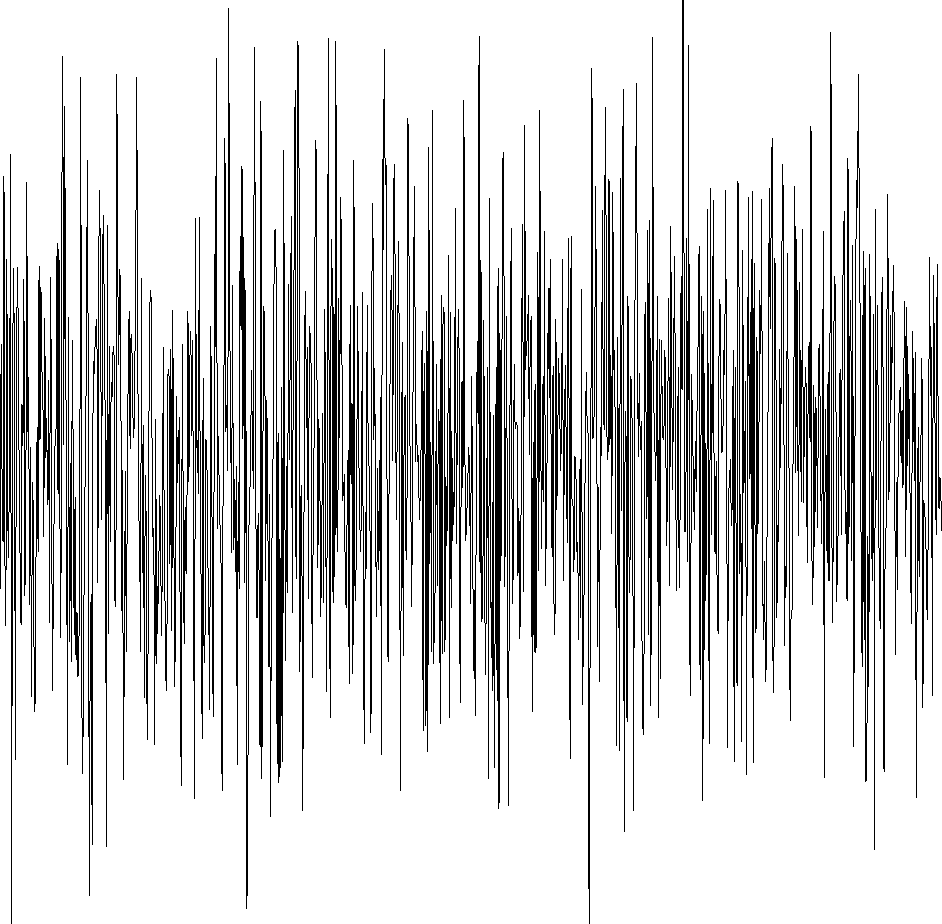
\includegraphics[width=\linewidth, keepaspectratio=false, height=.15\textheight]{noise.png}}
        \only<7>{Trame détecté $\vect{F}_D$ \\ "ZZZZZZZZ \Xb{}\Ob{}\Ob{}\Xb{}~\Xb{}\Ob{}?\Xb{}~\Ob{}??\Xb{}~\Ob{}\Ob{}\Xb{}\Ob{}~\Xb{}\Ob{}?\Xb{}~\Xb{}\Ob{}\Xb{}\Ob{} ZZZZZZZZZZZ"\\\vspace{1em} \Ob{}: +1 --- \Xb{}: -1 --- Z: Noise --- ?: Noisy Chip}
        \only<8>{Trame synchronisée $\vect{F}$ \\ "\Xb{}\Ob{}\Ob{}\Xb{}~\Xb{}\Ob{}?\Xb{}~\Ob{}??\Xb{}~\Ob{}\Ob{}\Xb{}\Ob{}~\Xb{}\Ob{}?\Xb{}~\Xb{}\Ob{}\Xb{}\Ob{}"\\\vspace{1em} \Ob{}: +1 --- \Xb{}: -1 --- ?: Noisy Chip}
      \end{column}
      \begin{column}{.04\linewidth} \centering
        \only<1-3>{$\Rightarrow$}
        \only<6->{$\Rightarrow$}
      \end{column}
      \begin{column}{.48\linewidth} \centering
        \only<1>{Mot de code $\vect{C}$ \\ "1 2 1 3 2 3"}
        \only<2>{Trame CCSK $\vect{F}_{CCSK}$ \\ "\Ob{}\Xb{}\Xb{}\Xb{}~\Xb{}\Ob{}\Xb{}\Xb{}~\Ob{}\Xb{}\Xb{}\Xb{}~\Xb{}\Xb{}\Ob{}\Xb{}~\Xb{}\Ob{}\Xb{}\Xb{}~\Xb{}\Xb{}\Ob{}\Xb{}"\\\vspace{1em} \Ob{}: 1 --- \Xb{}: 0\\CCSK Sequence: \Ob{}\Xb{}\Xb{}\Xb{}}
        \only<3>{Trame QCSP $\vect{F}\phantom{_{CCSK}}$ \\ "\Xb{}\Ob{}\Ob{}\Ob{}~\Xb{}\Ob{}\Xb{}\Xb{}~\Ob{}\Xb{}\Xb{}\Xb{}~\Ob{}\Ob{}\Xb{}\Ob{}~\Xb{}\Ob{}\Xb{}\Xb{}~\Ob{}\Ob{}\Xb{}\Ob{}"\\\vspace{1em} \Ob{} : +1 --- \Xb{} : -1}
        \only<6>{Trame détectée $\vect{F}_D$ \\ "ZZZZZZZZ \Xb{}\Ob{}\Ob{}\Xb{}~\Xb{}\Ob{}?\Xb{}~\Ob{}??\Xb{}~\Ob{}\Ob{}\Xb{}\Ob{}~\Xb{}\Ob{}?\Xb{}~\Xb{}\Ob{}\Xb{}\Ob{} ZZZZZZZZZZZ"\\\vspace{1em} \Ob{}: +1 --- \Xb{}: -1 --- Z: Noise --- ?: Noisy Chip}
        \only<7>{Trame synchronisée $\vect{F}_S$ \\ "\Xb{}\Ob{}\Ob{}\Xb{}~\Xb{}\Ob{}?\Xb{}~\Ob{}??\Xb{}~\Ob{}\Ob{}\Xb{}\Ob{}~\Xb{}\Ob{}?\Xb{}~\Xb{}\Ob{}\Xb{}\Ob{}"\\\vspace{1em} \Ob{}: +1 --- \Xb{}: -1 --- ?: Noisy Chip}
        \only<8>{Message décodé $\vect{M}'$ \\ "1 2 1"}
      \end{column}
    \end{columns}

    \vspace{5 em}

    \only<4-5>{\centering \vspace{-6 em} 
    Flux d'échantillons\\
    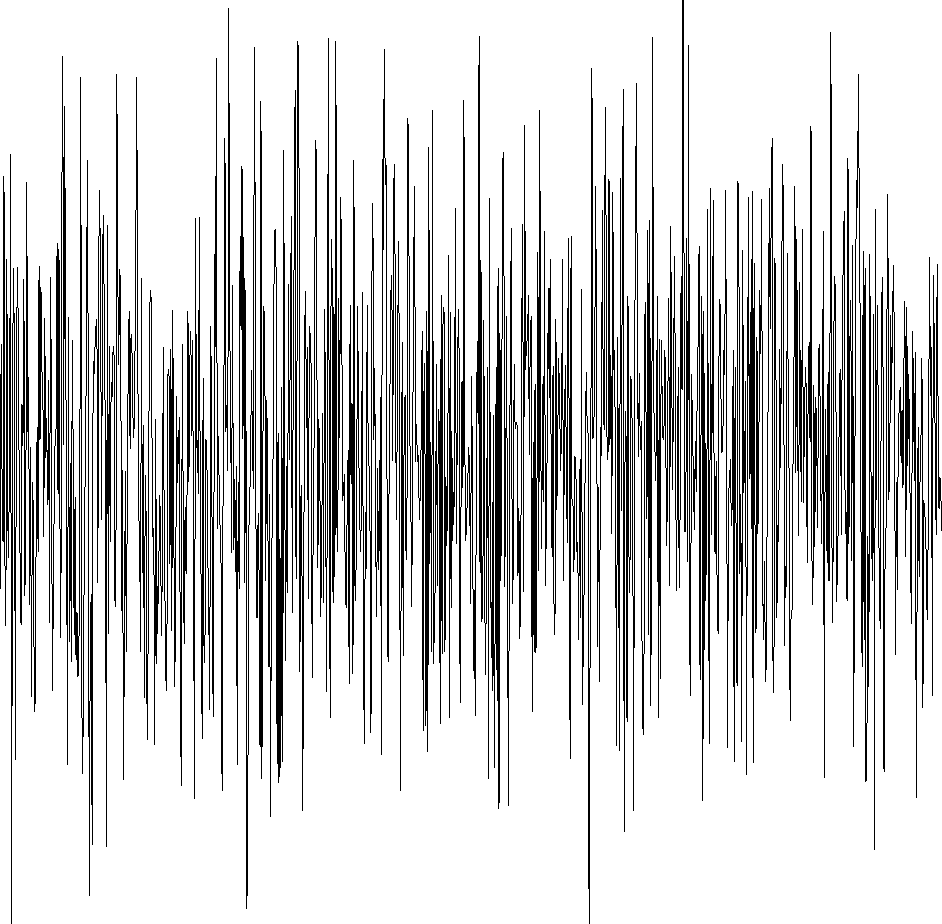
\includegraphics[width=\linewidth, keepaspectratio=false, height=.2\textheight]{noise.png}}
    \only<8>{\centering \vspace{-4 em} \scriptsize PS : La démodulation d'une trame QCSP produit des données directement utilisable par un décodeur NB-LDPC.}
  \end{overlayarea}
\end{frame}


\begin{frame}{\subsecname}
  \begin{center}
    \textcolor{RoyalBlue}{TODO, image de la chaine, et le canal théorique}
  \end{center}
\end{frame}

\subsection{Émission}


\begin{frame}{\subsecname}
  \begin{center}
    \textcolor{RoyalBlue}{TODO, les trois étape, et un filtre}
  \end{center}
\end{frame}

\subsection{Détection}

\begin{frame}{\subsecname : {Principe}}
  \begin{center}
    \textcolor{RoyalBlue}{TODO}
  \end{center}
\end{frame}


\begin{frame}{\subsecname : {animation CCSK demod}}
  \begin{center}
    \textcolor{RoyalBlue}{TODO}
  \end{center}
\end{frame}

\begin{frame}{\subsecname : {Problèmes Temps Fréquence}}
  \begin{center}
    \textcolor{RoyalBlue}{TODO}
  \end{center}
\end{frame}


\begin{frame}{\subsecname : {La grille temps fréquences}}
  \begin{center}
    \textcolor{RoyalBlue}{TODO}
  \end{center}
\end{frame}

\subsection{Synchronisation}

\begin{frame}{\subsecname}
  \begin{center}
    \textcolor{RoyalBlue}{TODO --- En fonction du temps, détails ou pas}
  \end{center}
\end{frame}

\subsection{Décodage}

\begin{frame}{\subsecname}
  \begin{center}
    \textcolor{RoyalBlue}{TODO --- Merci CCSK et hop}
  \end{center}
\end{frame}

\end{document}
